\section{Speed and Memory Footprint}
Implementing the technique of the previous section may be considered too costly.
First, it inserts many instructions before realizing most are useless, and copy
insertion is already by itself time-consuming. 
It introduces many new variables, too.
The size of the variable universe has an impact on the liveness analysis and
the interference graph construction. Also, if a general coalescing algorithm is used, a
graph representation with adjacency lists (in addition to the bit matrix) and a
working graph to explicitly merge nodes when coalescing variables, would be
required.  All these constructions, updates, manipulations are 
time-consuming and memory-consuming.  We may improve the whole process
by: a) avoiding the use of any interference graph and liveness sets; b) avoid the quadratic complexity of interference check between two sets of variables by an optimistic approach that first coalesces even interfering variables, then traverses each set of coalesced variables and un-coalesce one by one all the interfering ones\ifhab(this is the technique advocated by Budimlic et al. in~\cite{liverange.pldi02})\fi; c) emulating (``virtualizing'') the introduction of the
$\phi$-related copies.

\paragraph{Interference check}
Liveness sets and interference graph are the major source of memory usage. This motivates, in the context of JIT compilation, not to build any interference graph at all, and rely on the liveness check described in Chapter~\ref{chapter:ssa_tells_nothing_of_liveness} to test if two live-ranges intersect or not. Let us suppose for this purpose that a ``has-the-same-value'' equivalence relation, is available thanks to a mapping $V$ of variables to symbolic values: \\
$$\textrm{variables }a\textrm{ and }b\textrm{ have the same value } \Leftrightarrow V(a)=V(b)$$
As explained in Paragraph~\ref{par:alternative_ssa_destruction:value} this can be done linearly (without requiring any hash map-table) on a single traversal of the program if under strict SSA form. 
We also suppose that liveness check is available, meaning that for a given variable $a$ and program point $p$, one can answer if $a$ is live at this point through the boolean value of  $a.\textit{islive}(p)$. This can directly be used, under strict SSA form, to check is two variables live-ranges, say $a$ and $b$ intersect:
$$\begin{array}{rcl}
\intersect(a,b) & \Leftrightarrow & \textit{liverange}(a)\cap \textit{liverange}(b)\neq\emptyset\\
 & \Leftrightarrow & \left\lwave
\begin{array}{l}
\textit{a.def.op}=\textit{b.def.op}\\
\textit{a.def.op} \textrm{ dominates } \textit{b.def.op} \bigwedge \textit{a.islive}\left(\textit{out}(\textit{b.def.op})\right)\\
\textit{b.def.op} \textrm{ dominates } \textit{a.def.op} \bigwedge \textit{b.islive}\left(\textit{out}(\textit{a.def.op})\right)\\
\end{array}\right.
\end{array}
$$

Which leads to our refined notion of interference:

$$\interfere(a,b) \Leftrightarrow \intersect(a,b) \bigwedge V(a)\neq V(b)$$

\paragraph{De-coalescing in linear time}
The interference checking outlined in the previous paragraph allows to avoid building an interference graph of the SSA form program. However, coalescing has the effect of merging vertices and interference queries are actually to be done between sets of vertices. Using an interference graph, one can manipulate a \emph{working graph} which vertices corresponds to sets of coalesced variables, and update it along ongoing coalescing. Without any interference graph, one can ``naively'' test a quadratic number of interferences for each interference query. With more efforts\ifhab~\cite{Boissinot09}\fi, linear complexity is possible, but the technique considered here is even more radical. The idea is to first merge all copy and \phifun related variables together. A merged-set might of course contain interfering variables at this point. The idea is to identify some variables that interfere with some other variables within the merged-set, and remove them from the merged-set. As we will see here, thanks to the dominance property, this can be done linearly using a single traversal of the set.

In reference with register allocation, and graph coloring, we will associate the notion of colors to merged-sets: every variables of the same set are assigned the same color, and different sets are assigned different colors. The process of \emph{de-coalescing} a variable is to extract it from its set; it is not put in another set, just isolated. So we will refer such a variable as \emph{un-colored}. Actually, variables pinned together have to stay together. So the process of un-coloring a variable might have the effect of un-coloring some others. In other words, a colored variable is to be coalesced with variables of the same color, and any un-colored variable is to be coalesced only with the variables it is pinned with. 


We suppose that variables have already been colored and the goal is to un-color some of them (preferably not all of them) so that each merged-set become interference free. We suppose that if two variables are pinned together they have been assigned the same color, and that a merged-set cannot contain variables pinned to different physical resources. Here we focus on a single merged-set and the goal is to make it interference free within a single traversal. The idea\ifhab advocated by Budimlic et al.~\cite{Budimlic02} \fi exploits the tree shape of variables live-ranges under strict SSA. To this end, variables are identified by their definition point and ordered using dominance accordingly. Traversal of the set is performed along the dominance order, enforcing at each step the sub-set of already considered variables to be interference free. From now, we will abusively design as the dominators of a variable $v$, the set of variables of \emph{identical color than $v$} which definition dominate the definition of $v$. Variables defined at the same program point are arbitrarily ordered, so as to use the standard definition of immediate dominator (denoted $\cidom{v}$, set to $\undef$ if not exists).

First, consider the example of Figure~\ref{fig:alternative_ssa_destruction:fig:domtree} to illustrate the following properties. Consider the current variable $v$,  and an interfering dominating variable $\curanc$. Clearly, \curanc\ intersects (or is identical to) $\cidom{v}$: for our example, as $a$ does not intersect $\cidom{c}=b$ it cannot intersect $c$. On the other-end, with $e$ as the current variable, the intersection of $e$ with $a$ implies the intersection of $a$ with $\cidom{e}=d$. If by construction $d$ and $a$ do not interfere this implies that $V(a)=V(d)$... 
%
As a consequence, if one suppose that at a given step the set of dominating variables is interference free, checking if the current variable, say $v$, interferes with one of its dominating ones, consists in: (1) check if $v$ interfere with its immediate dominator, $u=\cidom{v}$; (2) if not, walk-up the dominators ($\curanc$) of $u$ that both intersect $u$ and have the same value $V$ than $u$: check the interference with $v$. Walking up along this set is done in Algorithm~\ref{alg:alternative_ssa_destruction:domup}, through the use of $\eanc{v}$ that points to the immediate dominating such variable. In this algorithm, we suppose that traversing the merged-set along the dominance order is possible, and that dominance test is available. As for the standard renaming pass during SSA construction, the $\textit{idom}$ field is set during the traversal as the updated value of \curidom.  


\begin{figure}
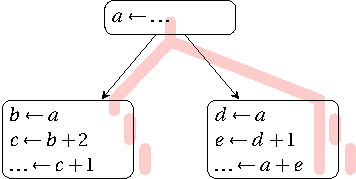
\includegraphics[width=0.6\textwidth]{domtree.pdf}
\caption{\label{fig:alternative_ssa_destruction:fig:domtree}Variables live-ranges are sub-trees of the dominator tree}
\end{figure}

\begin{algorithm}[h]
$\curidom=\undef$\;
\ForEach{variable $v$ of the merged-set in DFS pre-order of the dominance tree}{
  \tcc{Finds and set the immediate dominator of $v$}
  $u \gets \curidom$\;
  \While{$(u \neq \undef) \bigwedge \left(\neg(u \dominates\ v) \vee \uncolored(u)\right)$}{
         $u \gets \cidom{u}$\;
  }
  $\cidom{v}\gets u$\;
  $\curidom \gets v$\;
  \tcc{Walk up variables that have the same value than $u$\\
    Do it until $v$ is uncolored or no more interference with $v$} 
  $\eanc{v}\gets \undef$\;
  $\curanc \gets u$\;
  \While{$\curanc\neq\undef$}{
    \tcc{Find the first one that intersects $v$ with the same color than $u$}
    \While{$\curanc\neq \undef \bigwedge 
      \neg\left(\colored(\curanc) \wedge \intersect(\curanc,v)\right)$}{
      $\curanc \gets \eanc{\curanc}$\;
    }
    \If{$\curanc \neq \undef$}{
      \If{$V(\curanc) = V(v)$}{
	$\eanc{v} \gets \curanc$\;
	break \;
      }
      \Else { \tcc{$\curanc$ and $v$ interfere}
        \If{preferable to uncolor $v$}{
          uncolor $v$\;
          break\;
        } 
        \Else {
          uncolor $\curanc$\;
          $\curanc \gets \eanc{\curanc}$\;
        }
      }
    }
  }
}
\caption{\label{alg:alternative_ssa_destruction:domup} De-coalescing of a merged-set}
\end{algorithm}

\paragraph{Virtualizing $\phi$-related copies}
The last step toward a memory friendly and fast SSA-destruction algorithm consists in emulating the initial introduction of copies and only actually insert them on the fly when they appear to be required. We use \emph{exactly the same algorithms as for the solution without virtualization}, and use a special location in the code, identifies as a ``virtual'' parallel copy, where the real copies, if any, will be placed. 

Because of this, any non-coalesced split operand of a \phifun is assumed to have a use (resp. definition) in the parallel copy, and are then usually (unless used further) not considered as live-out (resp. live-in) of the corresponding basic-block. 
For any non-split operand, or when a virtual copy is coalesced, the use (resp. definition) operand is assumed (as in the multiplexing mode) to be at the exit (resp. entry) of the corresponding basic-block, so it is considered as live-out (resp. live-in). 
When the algorithm decides that a virtual copy $a'_i \gets a_i$ (resp. $a_0 \gets a'_0$)  cannot be coalesced, it is \emph{materialized} in the parallel copy and $a'_i$ (resp. $a'_0$) becomes explicit in its merged-set. 
The corresponding \phiop is replaced and the use of $a'_i$ (resp. def of $a'_0$) is now assumed, as in the multiplexing mode, to be on the corresponding control flow edge. 
This way, only copies that the first approach would finally leave un-coalesced are introduced. 


Without any virtualization, the process of transforming operand pining into live-range pining also introduces copies and new local variables pinned together. This systematic copy insertion can also be avoided and managed lazily just as for $\phi$-nodes isolation\ifhab (see Chapter~\ref{chapter:tree_scan} for an illustration)\fi. We will not address this aspect of the virtualization here: to simplify we consider any operand pining to be either ignored (handled by register allocation) or expressed as live-range pining.

In our scheme, every copy related (even virtual) variables are first coalesced (unless pining to physical resources forbid it), then merged-sets are traversed and interfering variables are de-coalesced.
A key implementation aspect is related to the handling of pining. In particular, for correctness purpose coalescing have to be performed in two separated steps. First pinned-$\phi$-webs have to be coalesced. Detection and fix of strong interferences is handled at this point. The so obtained merged sets (that contain local virtual variables) have to be identified as atomic i.e. they cannot be separated. After the second step of coalescing, atomic merged sets will compose larger merged sets. A variable cannot be de-coalesced from a set without de-coalescing its atomic merged-set from the set also. Non singletons atomic merged-sets have to be represented somehow. The trick is to use the \phifun itself as a placeholder for its set of local virtual variables: the pining of the virtual variables is represented through the pining of the corresponding \phifun. As a consequence, any \phifun will be pinned to all it non-split operands. 

Algorithm~\ref{alg:alternative_ssa_destruction:decoal} presents the process of de-coalescing with virtualization of $\phi$-related copies, using a single traversal of the whole program. Here each merged set is identified by a color. We suppose that the (interference free) atomic merged set containing a variable $v$ is available through the function $\atomic{v}$. $c.\curidom$ stores the last processed variable of color $c$. Just as for SSA renaming phase, thanks to $\cidom{u}$ link that points to the immediate dominator of variable $u$, the immediate dominator of the currently processed variable can be found. $\eanc{u}$ points to the lowest dominator of $u$ which live-range intersects $u$ and have the same value than $u$. Walking up along \textit{eanc} links allows to find the lowest dominator that intersects the current variable. 
A correctness subtlety is related to the interferences with a variable that is not yet materialized or coalesced. Either one need to ensure that they can be ignored or one need to emulate them. We choose to emulate them, which allows to postpone the materialization of all copies along a single traversal of the program at the really end of the de-coalescing process. As the live-range of a local virtual variable is very small starting (resp. ending for a $\phi$-definition operand) at the place of the parallel copy and ending at the exit (resp. starting at the entry) of the corresponding basic-block, the cases to consider is quite limited. A local virtual variable can interfere with a ``real'' variable $\curanc$, which is detected in Algorithm~\ref{alg:alternative_ssa_destruction:virtualdecoalesce} just as in Algorithm~\ref{alg:alternative_ssa_destruction:realdecoalesce}. It can also interfere with another virtual variable, the last processed being stored thanks to $c.\curphi$.
The materialization, is straightforward: whenever one of the two operands of a virtual copy is uncolored, or whenever the colors are different, the copy is materialized. This can be done through a single traversal of all \phifuns of the program.





\begin{algorithm}[h]
  \lForEach{$c\in \colors$}{$c.\curidom=\undef$; $c.\curphi=\undef$}\\
  \ForEach{basic-block $L$ in CFG in DFS pre-order of the dominance tree}{
    traverses all variables defined by an operation of L\;
    traverses all virtual variables defined by a \phifun of a successor of $L$\;
  }
  \caption{\label{alg:alternative_ssa_destruction:decoal} De-coalescing with virtualization of $\phi$-related copies}
\end{algorithm}

\begin{algorithm}[h]
    \ForEach{Operation $Op$ in $L$ in topological order (including \phifuns)}{
      \ForEach{variable $v$ defined by $Op$}{
        \lIf{$\neg\colored(v)$}{continue}
        \lElse{$c\gets \col(v)$}
        
        \tcc{Finds and set the immediate dominator of $v$}
        $u \gets c.\curidom$\;
        \While{$(u \neq \undef) \bigwedge \left(\neg(u \dominates\ v) \vee \neg\colored(u)\right)$}{
          $u \gets \cidom{u}$\;
        }
        $\cidom{v}\gets u$; $c.\curidom \gets v$\;
        
        \tcc{Walk up variables that have the same value than $u$} 
        $\eanc{v}\gets \undef$; $\curanc \gets u$\;
        \While{$\curanc\neq\undef$}{
          \tcc{Find the first one that intersects $v$ with the same color than $u$}
          \While{$\curanc\neq \undef \bigwedge 
            \neg\left(\colored(\curanc) \wedge \intersect(\curanc,v)\right)$}{
            $\curanc \gets \eanc{\curanc}$\;
          }
          \If{$\curanc \neq \undef$}{
            \If{$V(\curanc) = V(v)$}{
	      $\eanc{v} \gets \curanc$\;
	      break \;
            }
            \Else { \tcc{$\curanc$ and $v$ interfere}
              \If{preferable to uncolor $v$}{
                uncolor $\atomic{v}$\;
                break\;
              } 
              \Else {
                uncolor $\atomic{\curanc}$\;
                $\curanc \gets \eanc{\curanc}$\;
              }
            }
          }
        }      
      }
    }
\caption{\label{alg:alternative_ssa_destruction:realdecoalesce}Traverses all variables defined by an operation of L}
\end{algorithm}

\begin{algorithm}[h]
    \ForEach{basic-block $L'$ successor of $L$}{
      \ForEach{Operation $Phi:$ ``$L':a_0=\phi(\dots, L:a',\dots)$'' in $L'$}{
        \lIf{$\neg\colored(Phi)$}{continue}
        \lElse{$c\gets \col(Phi)$}
        
        \tcc{Finds and set the previous virtual variable of color $c$}
        $Phi'\gets c.\curphi$\;
        \If{$Phi'\neq \undef$}{
          \If{$L$ is a predecessor of the basic-block where $Phi'$ is defined}{
            $\curpred \gets \textsf{operand\_comming\_from\_L}(Phi')$
          } \Else {
            $c.\curphi\gets \undef$\;
            $Phi'\gets \undef$
          }
        }
        \If{$Phi'\neq\undef \wedge V(\curpred)\neq V(a')$}{ \tcc{Interference}
          uncolor $\atomic{Phi}$\;
          continue\;
        } \Else {
          $c.\curphi\gets Phi$
        }

        \tcc{Finds and set the immediate dominator of the local virtual variable}
        $u \gets c.\curidom$\;
        \While{$(u \neq \undef) \bigwedge \left(\neg(u \dominates\ L) \vee \neg\colored(u)\right)$}{
          $u \gets \cidom{u}$\;
        }
        $\cidom{v}\gets u$; 

        
        \tcc{Walk up variables that have the same value than $u$} 
        $\eanc{v}\gets \undef$; $\curanc \gets u$\;
        \While{$\curanc\neq\undef$}{
          \tcc{Find the first one that intersects $v$ with the same color than $u$}
          \While{$\curanc\neq \undef \bigwedge 
            \neg\left(\colored(\curanc) \wedge \curanc.\textit{islive}(\textit{out}(L))\right)$}{
            $\curanc \gets \eanc{\curanc}$\;
          }
          \If{$\curanc \neq \undef$}{ \tcc{$\curanc$ and $v$ interfere}
            \If{preferable to uncolor $Phi$}{
              uncolor $\atomic{Phi}$\;
              break\;
            } 
            \Else {
              uncolor $\atomic{\curanc}$\;
              $\curanc \gets \eanc{\curanc}$\;
            }
          }
        }

      }
    }
\caption{\label{alg:alternative_ssa_destruction:virtualdecoalesce}Traverses all virtual variables defined by a \phifun of a successor of L}

\end{algorithm}

        


\paragraph{Sequentialization of parallel copies}

                    
During the whole algorithm, we treat the copies placed at a given program point
as \emph{parallel copies}, which are indeed the semantics of $\phi$-functions.
This gives several benefits: a simpler implementation, in particular for
defining and updating liveness sets, a more symmetric implementation,
and fewer constraints for the coalescer. However, at the end of the process, we
need to go back to standard code, i.e., write the final copies in some
sequential order.

\ifhab
In most cases, a simple order of copies can be found, but sometimes more copies
are needed (more precisely, one for each cyclic permutation, with no
duplication) into one additional variable. Conceptually, the technique is
simple but it is more tricky to derive a fast implementation.  We designed a
fast sequentialization algorithm that requires the minimum number of copies.
We realized afterward that a similar algorithm has already been proposed by C.
May~\cite{May89}.

Nevertheless, for completeness, we give here a detailed description of
the algorithm as well as the complete pseudo-code
(Algorithm~\ref{alg:alternative_ssa_destruction_algorithm:para_copies_ser}).

Consider the directed graph~$G$ whose vertices are the variables
involved in the parallel copy and with an edge from $a$ to $b$
whenever there is a copy from~$a$ to $b$ (we write $a \mapsto
b$). This graph has the following key property: each vertex has a
unique incoming edge, the copy that defines it (a parallel copy $(b
\mapsto a, c \mapsto a)$ is possible but only if $V(b)=V(c)$ in which
case one of the copies can be removed). Thus, $G$ has a particular
structure: each connected component is a circuit (possibly reduced to
one vertex) and each vertex of the circuit can be the root of a
directed tree. The copies of the tree edges can be sequentialized
starting from the leaves, copying a variable to its successors before
overwriting it with its final value. Once these tree copies are
scheduled, it remains to consider the circuit copies. If at least one
vertex of the circuit was the root of a tree, it has already been
copied somewhere, otherwise, we copy one of the circuit vertices into
a new variable.  Then, the copies of the circuit can be
sequentialized, starting with the copy into this ``saved'' vertex and
back along the circuit edges. The last copy is done by moving the
saved value in the right variable. Thus, we generate the same number
of copies as expressed by the parallel copy, except possibly one
additional copy for each circuit with no tree edge, i.e., no
duplication of variable.  For example, for the parallel copy $(a
\mapsto b, b \mapsto c, c \mapsto a, c \mapsto d)$, there is one
circuit $(a,b,c)$ and an edge from $c$ to $d$, so we generate the
copies $d=c$, $c=a$, $a=b$, and $b=d$ (and not $b=c$).

Algorithm~\ref{alg:alternative_ssa_destruction_algorithm:para_copies_ser} emulates a traversal of $G$ (without
building it), allowing to overwrite a variable as soon as it is saved in some
other variable.  
\else
As explained in Section~\ref{sec:classical_construction_algorithm:destruction} (Algorithm~\ref{alg:ssadestruction:sequentialization}) the sequentialization of a parallel copy can be done using a simple traversal of a windmill farm shaped graph from the tip of the blades to the wheels. Algorithm~\ref{alg:alternative_ssa_destruction_algorithm:para_copies_ser} emulates a traversal of this graph (without building it), allowing to overwrite a variable as soon as it is saved in some
other variable.  
\fi

When a variable $a$ is copied in a variable $b$, the algorithm
remembers $b$ as the last location where the initial value of $a$ is available.
This information is stored into \texttt{loc}($a$). The initial value that
must be copied into $b$ is stored in \texttt{pred}($b$). The initialization
consists in identifying the variables whose values are not needed (tree
leaves), which are stored in the list \texttt{ready}.  The list
\texttt{to\_do} contains the destination of all copies to be treated.  Copies
are first treated by considering leaves (while loop on the list
\texttt{ready}). Then, the \texttt{to\_do} list is considered, ignoring
copies that have already been treated, possibly breaking a circuit with no
duplication, thanks to an extra copy into the fresh variable $n$.

\begin{algorithm}[h]
%\Input{A parallel copy $P$}
%\Blankline
%value $\leftarrow$ \texttt{new} hash table \;
%targets $\leftarrow$ \texttt{new} hash table \;
  \KwData{Set $P$ of parallel copies of the form $a \mapsto b$, $a \neq b$, one extra fresh variable $n$}
\KwOut{List of copies in sequential order}
ready $\leftarrow []$ ;
to\_do $\leftarrow []$ ; pred($n$) $\leftarrow \bot$ \;
\ForAll{$(a \mapsto b) \in P$}{
	loc($b$)$ \leftarrow \bot$ ; pred($a$) $\leftarrow \bot$ \tcc*{initialization}
}

\ForAll{$(a \mapsto b) \in P$}{
	loc($a$) $\leftarrow a$ \tcc*{needed and not copied yet}
	pred($b$) $\leftarrow a$ \tcc*{(unique) predecessor}
        to\_do.push($b$) \tcc*{copy into $b$ to be done}
}

\ForAll{$(a \mapsto b) \in P$}{
	\lIf{loc($b$) = $\bot$}{ready.push($b$) \tcc*{$b$ is not used and can be overwritten}
	}
}
\While{to\_do $\neq []$}{
	\While{ready $\ne []$}{
		$b \leftarrow$ ready.pop() \tcc*{pick a free location}
		$a \leftarrow$ pred($b$) ; $c \leftarrow$ loc($a$) \tcc*{available in $c$}
		\texttt{emit\_copy}($c \mapsto b$) \tcc*{generate the copy}
		loc($a$) $\leftarrow b$ \tcc*{now,
                  available in $b$}
                \lIf{$a=c$ and pred($a$) $\neq \bot$}{
                   ready.push(a) \tcc*{just copied, can be overwritten}}
%		\texttt{del}\ targets[$a$] \;
%		\If{$b \in$ targets.keys()}{
%			available.append($b$) \;
%		}
	}
%	\If{targets.keys() $\neq []$}{
        
        
        $b \leftarrow$ to\_do.pop() \tcc*{look for remaining copy}
        \If{$b =$ loc(pred($b$))}{
%
%

%        $a' \leftarrow$ \texttt{new\_ressource}() \;
          \texttt{emit\_copy}($b \mapsto n$) \tcc*{break circuit with copy}
		loc($b$) $\leftarrow n$ \tcc*{now, 
                  available in $n$}
                ready.push($b$) \tcc*{$b$ can be overwritten}
%         \If{$b \in$ targets.keys()}{
%           available.append($b$) \;
%         }
%         values[$b$] $\leftarrow a'$ \;
}
	
}
        \caption{Parallel copy sequentialization algorithm}
        \label{alg:alternative_ssa_destruction_algorithm:para_copies_ser}
\end{algorithm}
%% +Pour l'implémenter on différentie resources et valeurs . La copie a->b%% +signifie que la valeur dans la resource a doit être copiee dans la
%% +resource b.  On racourcit en disant que la valeur ``a'' initialement
%% +dans la resource ``a'' doit être copiee dans la resource
%% +``b''.\\ Ainsi on maintient pour chaque valeur (v) dans quelle
%% +resource elle est disponible (Rcur(v)) et pour chaque resource (r)
%% +quelle valeur (s'il y en a une) elle devra contenir à la fin (Vend(r))
%% +(predecesseur dans le graphe).\\ On construit initialement et
%% +maintient la liste des feuilles ``leaves'' ie de resources qui ne
%% +contiennent pas de valeur (où bien la valeur est disponible
%% +ailleur). On est pour cela obligé de parcourir la liste des valeurs et
%% +marquer les resource qui contiennent une valeur. \\ On construit une
%% +autre liste ``todo'' qui est la liste des resources qui doivent avoir
%% +une valeur à la fin et qui ne contiennent pas cette valeur.\\ Si
%% +leaves n'est pas vide on pull une feuille b, et donc une copie de a->b
%% +avec a=Rcur(Vend(b)). On génère cette copie, et on set
%% +Rcur(Vend(b)):=b (la valeur Vend(b) qui était dans a est maintenant
%% +dans b). a est donc libérée de la valeur Vend et on push  a dans
%% +leaves.\\ Si leaves est vide, c'est soit que c'est terminé, soit qu'il
%% +y a un cycle sans duplication. Dans ce cas, on pull une resource a. Si
%% +Rcur(Vend(a))==a, a a déjà été traité, on passe. Sinon, on est en
%% +présence d'un cycl avec Rcur(a)=a. on génère une nouvelle variable
%% +(resource) a', on genère la copie a->a'. On met à jour Rcur(a):=a'. A
%% +est libéré, on le met dans leaves.
